\documentclass[11pt, a4paper]{article}
\usepackage{graphicx}
\usepackage{amsmath}
\usepackage{listings}
\usepackage{minted}

\title{EE2703 Applied Programming Lab - Assignment No 4}
\author{
  \textbf{Name}: Atishay Ganesh\\
  \textbf{Roll Number}: EE17B155
}\date{\today}
\begin{document}
		
\maketitle 
\section{Abstract}
The goal of this assignment is the following.
\begin{itemize}
\item To fit two functions $e^{x}$ and $cos(cos(x))$ using the Fourier series.
\item To use least squares fitting to simplify the process of calculating Fourier series.
\item Studying the effect of discontinuities on the Fourier Series, and the Gibbs Phenomenon.
\item To plot graphs to understand the above
\end{itemize}
\usemintedstyle{manni}

\section{Assignment}
\subsection{Part 1}
Importing the standard libraries
\begin{minted}[mathescape,escapeinside = ||]{python3}
import numpy  as np
import matplotlib.pyplot as plt
import scipy.integrate
\end{minted}
Defining the functions $e^{x}$ and $cos(cos(x)$
\begin{minted}{python3}
def exp(x):
    return np.exp(x)

def coscos(x):
    return np.cos(np.cos(x))
\end{minted}
We define a plotting function to help simplify the code.
\begin{minted}{python3}
def plotter(fig_no,plot_x,plot_y,label_x,label_y,type=None,kind='b-',title=""):
    plt.figure(fig_no)
    plt.grid(True)
    if type =="semilogy":
        plt.semilogy(plot_x,plot_y,kind)
    elif type =='ll':
        plt.loglog(plot_x,plot_y,kind)
    elif type ==None:
        plt.plot(plot_x,plot_y,kind)
    plt.xlabel(label_x,size =19)
    plt.ylabel(label_y,size =19)
    plt.title(title)
\end{minted}
We evaluate the functions from $-2\pi$ to $4\pi$ to plot, and we also plot a periodic extension of the functions.
\begin{minted}{python3}
t = np.linspace(-2*np.pi,4*np.pi,1200)
fr_length = np.arange(1,52)#Fourier Coefficient Number

plotter(1,t,exp(t),r"$t$",r"exp(t)",
"semilogy",title ="Exponential Function on a semilog plot")
plotter(2, t, coscos(t)), r"$t$", r"cos(cos(t))",
title="Cos(Cos(t)) Function on a linear plot")
plotter(1, t,
np.concatenate((exp(t)[400:800], exp(t)[400:800], exp(t)[400:800])),
r"$t$", r"exp(t)", "semilogy", 'r-')
plt.legend(("true","periodic extension"))
plotter(2, t,
np.concatenate((coscos(t)[400:800], coscos(t)[400:800], coscos(t)[400:800])),
r"$t$", r"exp(t)", "semilogy",'r-')
plt.legend(("true","periodic extension"))
\end{minted}

\begin{figure}[!tbh]
   	\centering
   	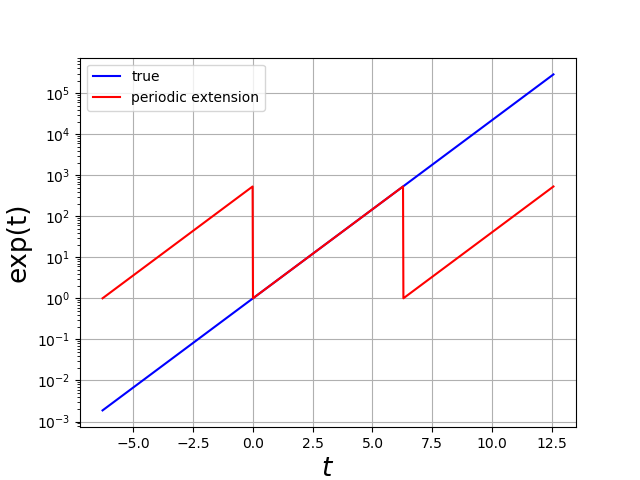
\includegraphics[scale=0.5]{Figure_11.png}
   	\label{fig:11}
   	\caption{$e^{t}$ vs t on a linear plot}
   \end{figure}
\begin{figure}[!tbh]
   	\centering
   	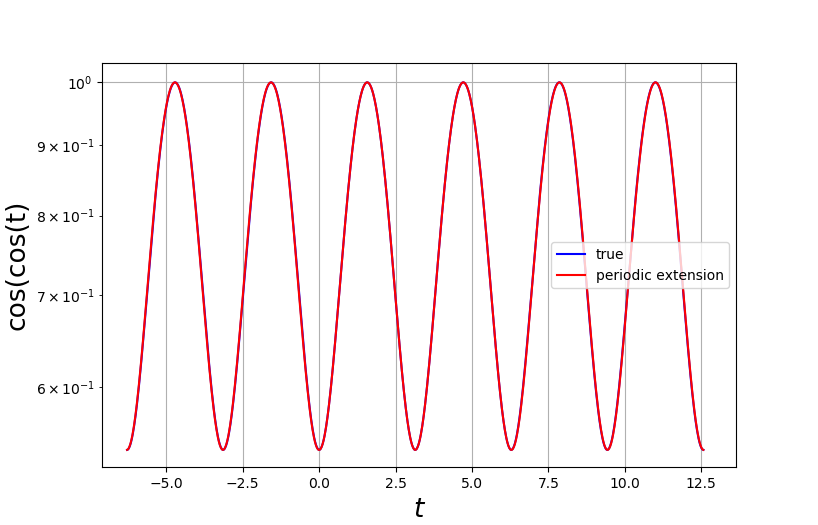
\includegraphics[scale=0.5]{Figure_21.png}
   	\label{fig:21}
   	\caption{$cos(cos(t))$ vs t on a linear plot}
   \end{figure}

\subsection{Part 2}
We use the integrator in scipy to calculate the fourier integrals in a for loop.
And then we plot them.
\begin{minted}{python3}
def u1(x,k):
    return(coscos(x)*np.cos(k*x))

def v1(x,k):
    return(coscos(x)*np.sin(k*x))

def u2(x,k):
    return(exp(x)*np.cos(k*x))

def v2(x,k):
    return(exp(x)*np.sin(k*x))


def integrate():
    a = np.zeros(51)
    b = np.zeros(51)
    a[0] =  scipy.integrate.quad(exp,0,2*np.pi)[0]/(2*np.pi)
    b[0] =  scipy.integrate.quad(coscos,0,2*np.pi)[0]/(2*np.pi)
    for i in range(1,51,2):
        a[i] = scipy.integrate.quad(u2,0,2*np.pi,args=(i//2+1))[0]/(np.pi)
        b[i] = scipy.integrate.quad(u1,0,2*np.pi,args=(i//2+1))[0]/(np.pi)
        a[i+1] = scipy.integrate.quad(v2,0,2*np.pi,args=(i//2+1))[0]/(np.pi)
        b[i+1] = scipy.integrate.quad(v1,0,2*np.pi,args=(i//2+1))[0]/(np.pi)
    return a,b

frexp,frcos = integrate()
\end{minted}
\subsection{Part 3}

And now we plot the Fourier series terms.

\begin{minted}{python3}
plotter(3,fr_length,
np.absolute(frexp),"Coefficient Number",
"Coefficient Value","semilogy",'ro',
title="Semilog Fourier Coefficients for exp(t)")
plotter(4,fr_length,
np.absolute(frexp),"Coefficient Number",
"Coefficient Value","ll",'ro',
title="Log-Log Fourier Coefficients for exp(t)")
plotter(5,fr_length,
np.absolute(frcos),"Coefficient Number",
"Coefficient Value","semilogy",
'ro',title="Semilog Fourier Coefficients for coscos(t)")
plotter(6,fr_length,
np.absolute(frcos),"Coefficient Number",
"Coefficient Value","ll",'ro',
title="Loglog Fourier Coefficients for coscos(t)")
plt.show()
\end{minted}

\begin{figure}[!tbh]
   	\centering
   	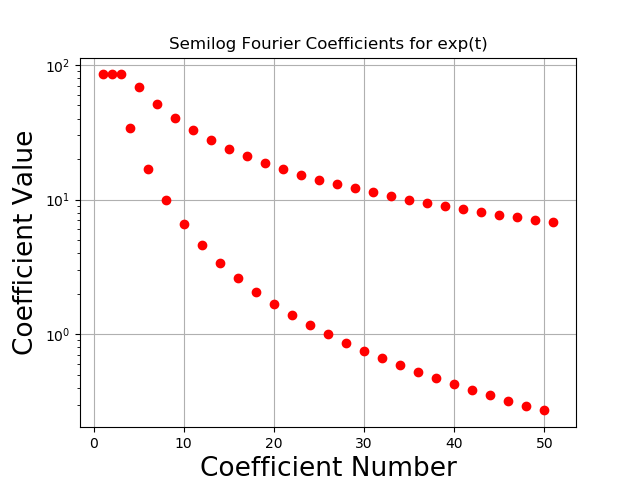
\includegraphics[scale=0.5]{Figure_31.png}
   	\label{fig:11}
   \end{figure}
\begin{figure}[!tbh]
   	\centering
   	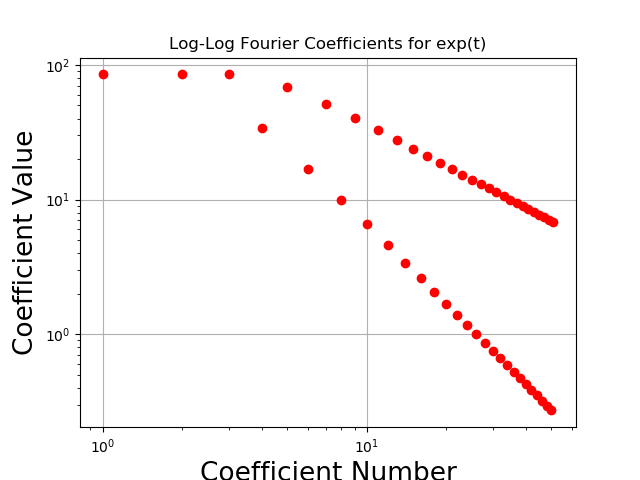
\includegraphics[scale=0.5]{Figure_41.png}
   	\label{fig:21}
   \end{figure}
   
\begin{figure}[!tbh]
   	\centering
   	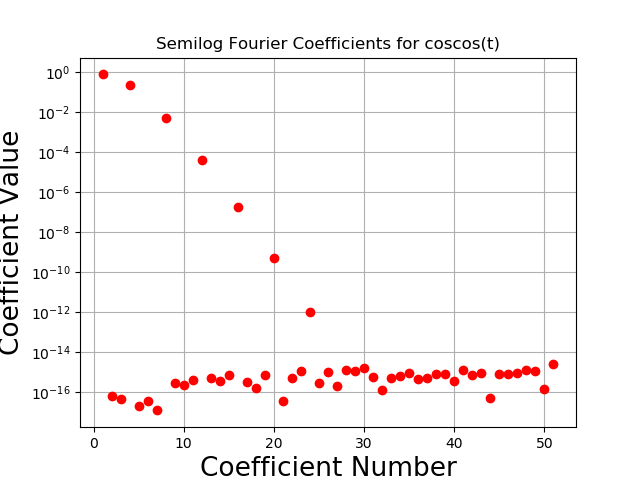
\includegraphics[scale=0.5]{Figure_51.png}
   	\label{fig:11}
   \end{figure}
\begin{figure}[!tbh]
   	\centering
   	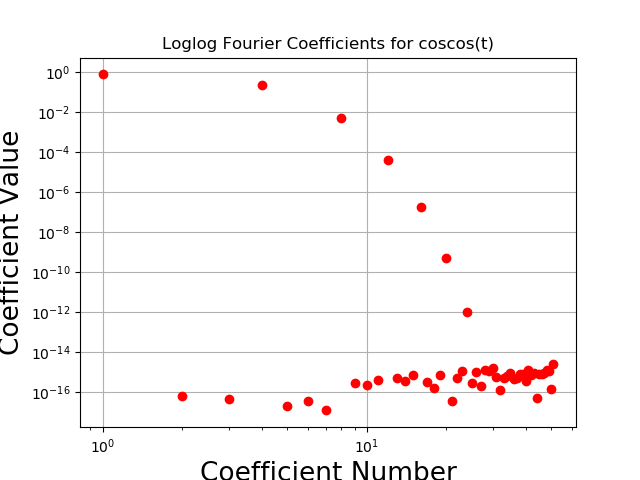
\includegraphics[scale=0.5]{Figure_61.png}
   	\label{fig:21}
   \end{figure}

{$a.$ The $b_{n}$ coefficients are nearly zero for $cos(cos(t))$ since it is an even function, and hence does not have an odd component.}
\\
{b. The magnitude of the coefficients would represent how much of certain frequencies happen to be in the output. $cos(cos(t))$ does not have very many frequencies of harmonics, so it dies out quickly. However, since the periodic extension of $e^{t}$ is discontinuous. To represent this discontinuity as a sum of continuous sinusoids, we would need high frequency components, hence coefficients do not decay as quickly.}
\\
{c. The loglog plot is linear for $e^{t}$ since Fourier coefficients of $e^{t}$ decay with $1/n$ or $1/n^{2}$. The semilog plot seems linear in the $cos(cos(t))$ case as its fourier coefficients decay exponentially with n.
}

\subsection{Parts 4 and 5}
We now use a least squares approach to calculate the Fourier series.
\begin{minted}{python3}
x =np.linspace(0,2*np.pi,400,endpoint =True)
bexp = exp(x)
bcoscos =coscos(x)
A = np.zeros((400,51))
A[:,0] =1
for k in range(1,26):
    A[:,2*k-1] = np.cos(k*x)
    A[:,2*k] = np.sin(k*x)
cexp = np.linalg.lstsq(A,bexp)[0]
ccoscos = np.linalg.lstsq(A,bcoscos)[0]
cexp = np.linalg.lstsq(A,bexp)[0]
ccoscos = np.linalg.lstsq(A,bcoscos)[0]

plotter(3,fr_length,np.abs(cexp),"Coefficient Number",
"Coefficient Value","semilogy",'go',
title="Semilog Fourier Coefficients for exp(t)")
plt.legend(("true","predicted"))
plotter(4,fr_length,np.abs(cexp),"Coefficient Number",
"Coefficient Value","ll",'go',
title="Loglog Fourier Coefficients for exp(t)")
plt.legend(("true","predicted"))
plotter(5,fr_length,np.abs(ccoscos),"Coefficient Number",
"Coefficient Value","semilogy",'go',
title="Semilog Fourier Coefficients for coscos(t)")
plt.legend(("true","predicted"))
plotter(6,fr_length,np.abs(ccoscos),"Coefficient Number",
"Coefficient Value","ll",'go',
title="Loglog Fourier Coefficients for coscos(t)")
plt.legend(("true","predicted"))
\end{minted}


\begin{figure}[!tbh]
   	\centering
   	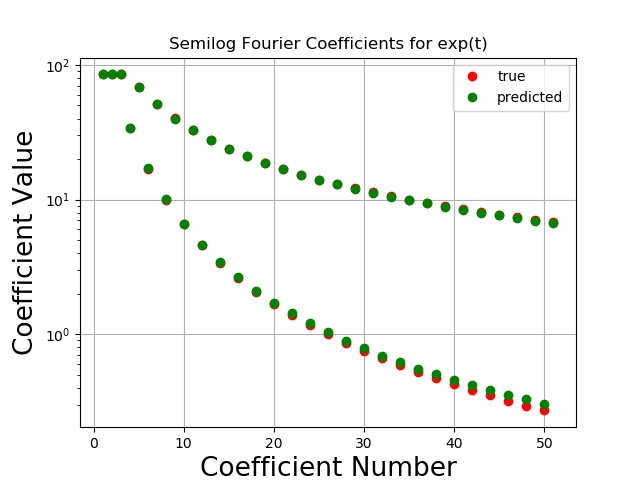
\includegraphics[scale=0.5]{Figure_32.png}
   	\label{fig:32}
   \end{figure}
\begin{figure}[!tbh]
   	\centering
   	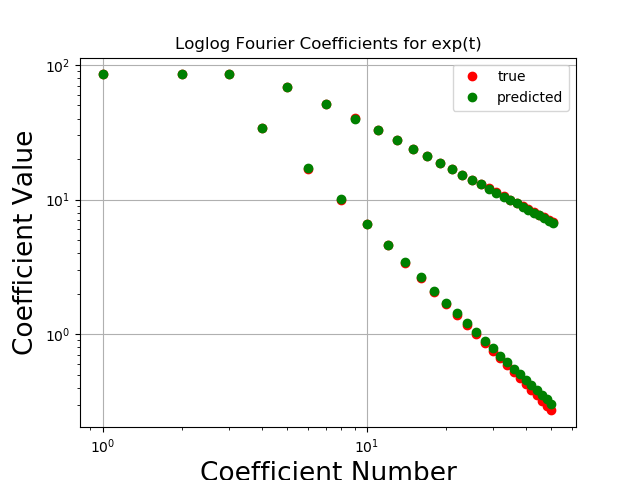
\includegraphics[scale=0.5]{Figure_42.png}
   	\label{fig:42}
   \end{figure}
\begin{figure}[!tbh]
   	\centering
   	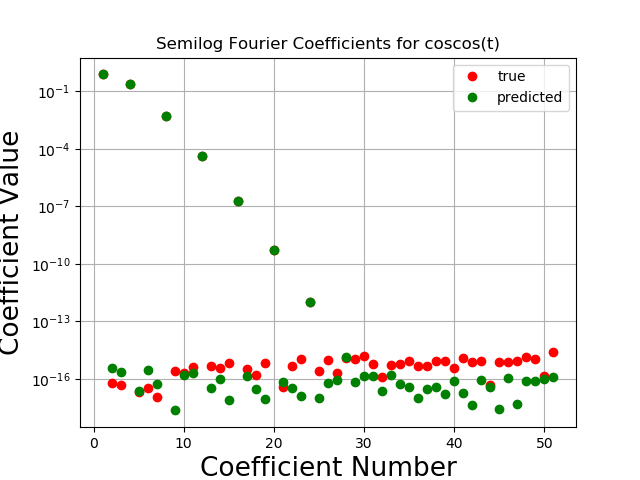
\includegraphics[scale=0.5]{Figure_52.png}
   	\label{fig:52}
   \end{figure}
\begin{figure}[!tbh]
   	\centering
   	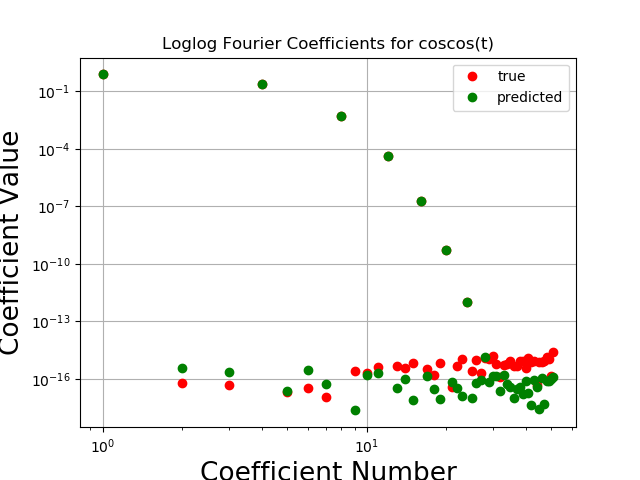
\includegraphics[scale=0.5]{Figure_62.png}
   	\label{fig:62}
   \end{figure}

\subsection{Part 6}
We can find the absolute difference between the two answers by subtracting the two vectors in vector form, take the absolute value and finding the maximum.
\begin{minted}{python3}
diffexp = np.absolute(cexp-frexp)
diffcos = np.absolute(ccoscos-frcos)
print(np.amax(diffexp),np.amax(diffcos))
\end{minted}
{0.0881216977876722 2.5466388061776397e-15
}
\\
\\
{There is very good agreement in values in the case of $cos(cos(x))$ but a significant amount of difference in the case of $e^{t}$. The reason for this is that the periodic extension of the exponential function is discontinuous, and hence would require a lot more samples to accurately determine its Fourier coefficients. If we increased the number of samples to $10^{6}$, the maximum deviation would reduce, but not vanish.
The effect of this lack of samples is felt more near the discontinuity of the signal, which can be attributed to the Gibbs Phenomenon.
}
\subsection{Part 7}
The function is evaluated using the fourier coefficients calculated via the least squares method.
\begin{minted}{python3}
Acexp = A@cexp
Accos = A@ccoscos
plotter(1,t,np.concatenate((np.zeros(400),Acexp,np.zeros(400))),
r"$t$",r"exp(t)","semilogy",'go')
plt.legend(("true","periodic extension","predicted"))
plotter(2,t,np.concatenate((np.zeros(400),Accos,np.zeros(400))),
r"$t$",r"coscos(t)",None,'go')
plt.legend(("true","periodic extension","predicted"))
\end{minted}
{The $cos(cos(t))$ vs t graph, agrees almost perfectly, beyond the scope of the precision of the least squares fitter.
The Fourier approximation of $e^{t}$ does not agree very well to the ideal case near the discontinuity. The cause for this is the Gibbs Phenomenon, which can be described as below.
The partial sums of the Fourier series will have large oscillations near the discontinuity of the function. These oscillations do not die out as n increases, but approaches a finite limit.
This is one of the causes of ringing artifacts in signal processing, and is very undesirable.
Plotting the output on a linear graph would make this ringing much more apparent.
}
\begin{figure}[!tbh]
   	\centering
   	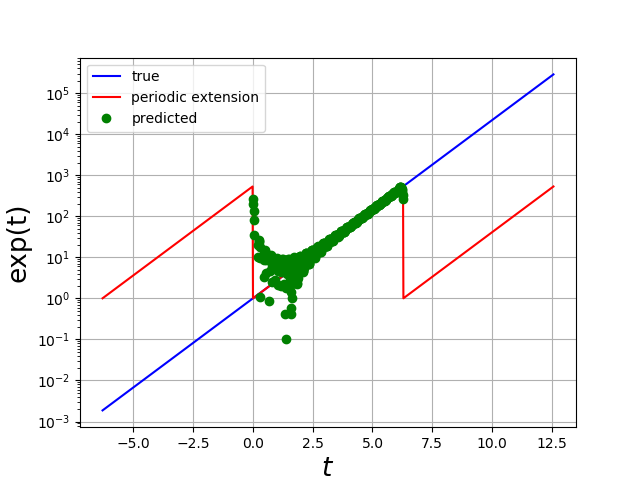
\includegraphics[scale=0.5]{Figure_12.png}
   	\caption{$e^{t}$ vs t on a linear plot}

   	\label{fig:32}
   \end{figure}
\begin{figure}[!tbh]
   	\centering
   	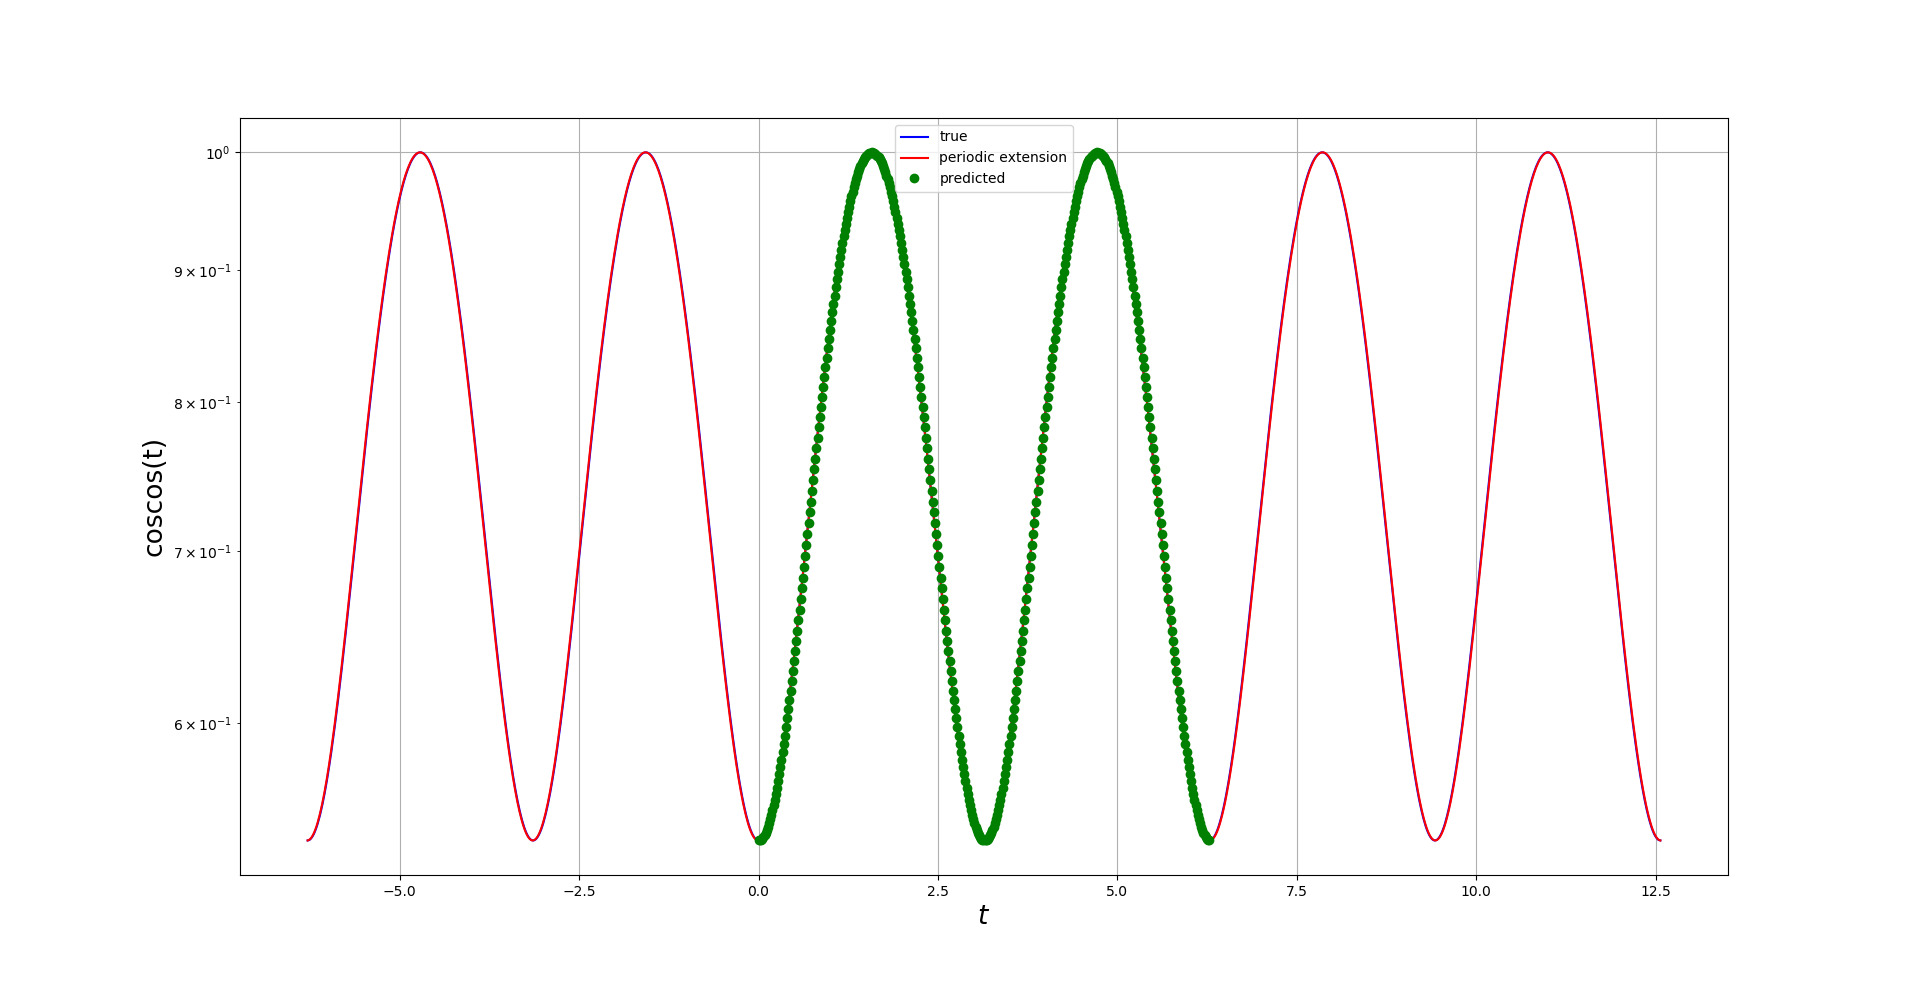
\includegraphics[scale=0.25]{Figure_22.png}
   	\label{fig:42}
   	\caption{$cos(cos(t))$ vs t on a linear plot}

   \end{figure}
\section{Conclusions}
\begin{itemize}
\item We saw two different ways to calculate the Fourier series of a periodic signal.
\item We saw how least squares fitting can be used to simplify the process of calculating the Fourier Series.
\item We observed Gibbs phenomenon at the discontinuity in the Fourier approximation of $e^{t}$.
\end{itemize}

\end{document}



 